\section{Meta-Decompositions}
\label{sec:meta}

Even though we have shown a connection between join trees and width-1 query plans in \cref{thm:w1plan-size-bound} and \cref{thm:w1plan-jt}, it is impractical to find the optimal width-1 query plan by enumerating every possible join tree---As noted earlier, a query can have an exponential number of possible join trees. Therefore, in this section, we introduce and explore a generalized representation that efficiently captures all join trees of an acyclic query. This enables us to optimize queries directly on this representation, eliminating the need to enumerate all possible join trees. 

We highlight an observation that \emph{the exponential number of possible join trees often arises when multiple relations share common join attributes}, as is the case for star queries discussed in \cref{thm:exp-join-trees} and illustrated by \cref{ex:star}.
In such a query, any pair of relations has valid join predicates, so in join trees of such queries, these relations can be connected in any arbitrary tree structure.
% , meaning there are $\tbinom{n}{2} = \frac{n(n-1)}{2}$ pairwise predicates. Any specific join tree selects only $n-1$ of those predicates and infers the remaining predicates through the tree structure, where $\frac{(n-1)(n-2)}{2}$ predicates are not selected for that particular tree.
On the contrary, in the case of a query like in \cref{ex:hierarchical}, where the join attributes are unique for all possible pairs of relations to be joined, the query demonstrates a more ``tree-like'' structure.  There is a unique tree structure for such a query, with $n$ distinct, structurally isomorphic join trees, differing only by the choice of the root relation.

In light of this, we introduce \emph{meta-decompositions}. In the case of acyclic conjunctive queries, they can capture all possible join trees but require only linear space.
One of the major differences from standard join trees is the addition of ``minor nodes'' to handle cases when more than two relations share the same join key.
These nodes have empty $\lambda$-labels, meaning they are not associated with a single relation, but their $\chi$-labels contain the shared join keys.
Additionally, we add a $\kappa$-label to each node to denote the ``interface'' with the remaining relations of the join tree that are not in the subtree rooted at the node.
\begin{example}
    The meta-decomposition of the query $Q_{\ref{ex:star}}$ in \cref{ex:star} is shown in \cref{fig:star-meta}. The root of this tree is a minor node, showing that the four children share precisely the attribute $x_1$. Note also that the $\kappa$-label of all 4 non-root nodes is exactly $\{ x_1 \}$.
\end{example}
\begin{example}
    The meta-decomposition of the query $Q_{\ref{ex:hierarchical}}$ in \cref{ex:hierarchical} is shown in \cref{fig:hierarchical-meta}. It has the exact same structure as the join tree shown in \cref{fig:hierarchical-jt} and has no minor node, as all pairs of relations have different intersections of attributes.
\end{example}
\begin{figure*}
    \begin{minipage}[b]{0.48\linewidth}
    \centering
    \small
    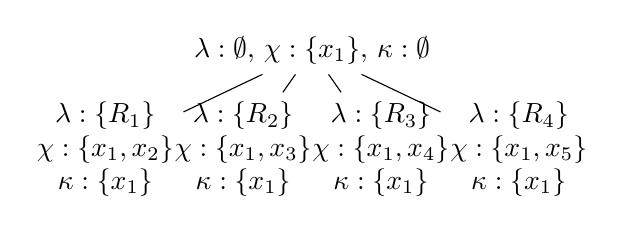
\begin{tikzpicture}[
        level distance=1.25cm,
        level 1/.style={sibling distance=1.75cm},
    ]
    \node[align=center] { $\lambda: \emptyset$, $\chi: \{ x_1 \}$, $\kappa: \emptyset$} 
        child { node [align=center] {$\lambda: \{ R_1 \}$ \\ $\chi: \{ x_1, x_2 \}$ \\ $\kappa: \{ x_1 \}$ } edge from parent[-] }
        child { node [align=center] { $\lambda: \{ R_2 \}$ \\ $\chi: \{ x_1, x_3 \}$ \\ $\kappa: \{ x_1 \}$ } edge from parent[-] }
        child { node [align=center] { $\lambda: \{ R_3 \}$ \\ $\chi: \{ x_1, x_4 \}$ \\ $\kappa: \{ x_1 \}$ } edge from parent[-] }
        child { node [align=center] { $\lambda: \{ R_4 \}$ \\ $\chi: \{ x_1, x_5 \}$ \\ $\kappa: \{ x_1 \}$ } edge from parent[-] }
    ;
    \end{tikzpicture}
    \captionof{figure}{Meta-decomposition of the query $Q_{\ref{ex:star}}$}
    \label{fig:star-meta}
\end{minipage}
    \hfill
    \begin{minipage}[b]{0.48\linewidth}
    \centering
    \small
    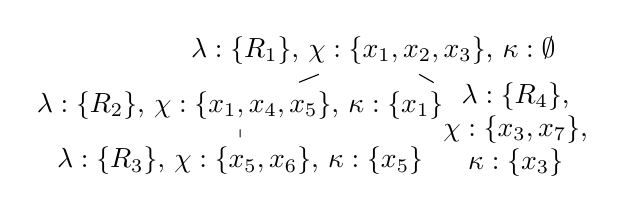
\begin{tikzpicture}[
			level distance=0.7cm,
			level 1/.style={sibling distance=3.5cm}
        ]
        \node[align=center] { $\lambda: \{ R_1 \}$, $\chi: \{ x_1, x_2, x_3 \}$, $\kappa: \emptyset$ }
            child[align=center] { node {$\lambda: \{ R_2 \}$, $\chi: \{ x_1, x_4, x_5 \}$, $\kappa: \{ x_1 \}$} edge from parent[-]
                child[align=center] { node {$\lambda: \{ R_3 \}$, $\chi: \{ x_5, x_6 \}$, $\kappa: \{ x_5 \}$} edge from parent[-] }
            }
            child[align=center,level distance=1cm] { node {$\lambda: \{ R_4 \} $,\\$\chi: \{ x_3, x_7 \}$,\\$\kappa: \{ x_3 \}$} edge from parent[-]
            } ;
    \end{tikzpicture}
    \captionof{figure}{Meta-decomposition of the query $Q_{\ref{ex:hierarchical}}$}
    \label{fig:hierarchical-meta}
\end{minipage}
\end{figure*}

The formal definition is given as follows.


\begin{definition}
    Given a conjunctive query $Q$ and the associated hyergraph $H$, its \emph{meta-decomposition} $M = (V(M), r(M), E(M), \lambda, \chi, \kappa)$ is a labeled tree, where
    \begin{itemize}[leftmargin=*]
        \item $V(M)$ is the set of vertices, $r(M) \in V(M)$ is the root, and $E(M)$ is the set of edges,
        \item $\lambda : V(M) \rightarrow 2^{E(H)}$ maps each vertex of $M$ to a set of hyperedges of $H$ (possibly empty), and
        \item $\chi : V(M) \rightarrow 2^{V(H)}$ and $\kappa : V(M) \rightarrow 2^{V(H)}$ each maps each vertex of $M$ to a set of vertices of $H$,
    \end{itemize}
    such that it satisfies \ref{H1}, \ref{H2}, and
    \begin{enumerate}[label=(C\textsubscript{\arabic*}),ref=(C\textsubscript{\arabic*}),leftmargin=*]
        \setcounter{enumi}{3}
        \item[{\crtcrossreflabel{(C$_3'$)}[H3']}] For all $p \in V(M)$, $\chi(p) \subseteq V(\lambda(p))$ if $\lambda(p) \neq \emptyset$.
        \item\label{H4}\gdef\Giref{\ref{H4}} \textbf{Interface condition.} For every non-root $p \in V(M)$, let $q$ be $p$'s parent node. $\kappa(p)$ satisfies
        \begin{enumerate}
            \item $\kappa(p) = \chi(p) \cap \chi(V(M) \setminus V(M_p)) \subseteq \chi(q)$, where $M_p$ is the subtree of $M$ rooted at $p$; and
            \item $\kappa(p) \nsubseteq \chi(s) \text{ for all } s \in V(M) \setminus V(M_q)$ if $\kappa(p) \neq \chi(q)$.
        \end{enumerate}
        For the root node $r(M)$, we set $\kappa(r(M)) = \emptyset$.
        
        \item\label{H5}\gdef\Giref{\ref{H5}} \textbf{Minor nodes and uniqueness condition.} For every maximal subset of nodes $S = \{ p_1, \dots, p_n \} \subseteq V(M) $ $(n \geq 2)$ such that $ \kappa(p_1) = \dots = \kappa(p_n) = \kappa $ for some value of $\kappa$, there exists one unique node $ m \in V(M) $ with $ \lambda(m) = \emptyset $ and $ \chi(m) = \kappa$.
    \end{enumerate}
\end{definition}

In this paper, we consider acyclic queries and their ``minimal-width'' (``width-1'') meta-decompositions, which satisfy
\begin{enumerate}[label=(C\textsubscript{\arabic*}),ref=(C\textsubscript{\arabic*}),leftmargin=*]
    \setcounter{enumi}{3}
    \item[{\crtcrossreflabel{(C$_3''$)}[H3'']}] For all $p \in V(M)$ such that $\lambda(p) \neq \emptyset$, we have $|\lambda(p)| = 1$ and, w.l.o.g, $\chi(p) = V(\lambda(p))$.
\end{enumerate}

Besides introducing minor nodes in condition \ref{H5} and defining $\kappa$ as the interface in condition \ref{H4}(a), we also include condition \ref{H4}(b) that limits the shape of the meta-decomposition $M$: There can be multiple nodes that can satisfy $\kappa(p) \subseteq \chi(q)$, while condition \ref{H4}(b) limits $q$ to be the highest node with $\kappa(p) \subseteq \chi(q)$. We illustrate this with the following example:

\begin{example} \label{ex:meta-complicated}
    Consider the query
    \begin{align*}
        Q_{\ref{ex:meta-complicated}} \gets\ & R_1[x_1, x_2, x_6] \bowtie R_2[x_1, x_2, x_3, x_7] \bowtie R_3[x_1, x_3, x_4, x_8]
        \bowtie R_4[x_1, x_4, x_9] \bowtie R_5[x_1, x_{5}]
    \end{align*}
    Its hypergraph and meta-decomposition are shown in \cref{fig:complicated-hg} and \cref{fig:complicated-meta}, respectively.
    \cref{fig:complicated-jt1} and \cref{fig:complicated-jt2} show two valid join trees of this hypergraph. We highlight that $R_5$ could in fact be the child of any other node of the join tree, because its only interface with the rest of the hypergraph is $\{ x_1 \}$. For example, \cref{fig:complicated-jt3} is also a valid join tree.
    But, for the meta-decomposition in \cref{fig:complicated-meta}, according to condition \ref{H4}(b), we make $R_5$ the child of the highest possible node that contains $x_1$, which in this case is the root node, i.e., the minor node with $\chi$-label $\{ x_1, x_3 \}$.
    
    \begin{figure}
    \centering
    \begin{minipage}[b]{0.36\linewidth}
    \begin{subfigure}{\linewidth}
        \centering
        \begin{tikzpicture}[hypergraph,xscale=1.2,yscale=1.2]
            \node[vertex,label={east:$x_1$}] (x1) at (0, 0) {};
            \node[vertex,label={south:$x_2$}] (x2) at (0, -1) {};
            \node[vertex,label={north:$x_3$}] (x3) at (0, 1) {};
            \node[vertex,label={north:$x_4$}] (x4) at (-1, 0) {};
            \node[vertex,label={east:$x_5$}] (x5) at (1, 0) {};

            \node[vertex,label={south:$x_6$}] (x6) at (0, -2) {};
            \node[vertex,label={north:$x_7$}] (x7) at (0, 2) {};
            \node[vertex,label={north:$x_8$}] (x8) at (-1, 1) {};
            \node[vertex,label={east:$x_9$}] (x9) at (-2, 0) {};
        
            \begin{scope}[on background layer]
                
                \newcommand*{\pathri}{($(x1) + (0,0.5)$)
                    to[out=0,in=0] ($(x6) + (0,-0.5)$)
                    to[out=180,in=180] ($(x1) + (0,0.5)$)
                }
                    
                \newcommand*{\pathrii}{($(x7) + (0,0.6)$)
                    to[out=0,in=90] ($(x7) + (0.5,0)$)
                    to[out=-90,in=90] ($(x2) + (0.5,0)$)
                    to[out=-90,in=0] ($(x2) + (0,-0.6)$)
                    to[out=180,in=-90] ($(x2) + (-0.5,0)$)
                    to[out=90,in=-90] ($(x7) + (-0.5,0)$)
                    to[out=90,in=180] ($(x7) + (0,0.6)$)
                }
                
                \newcommand*{\pathriii}{($(x1) + (0.3,-0.3)$)
                    to[out=45,in=-45] ($(x3) + (0.3,0.3)$)
                    to[out=135,in=45] ($(x8) + (-0.3,0.3)$)
                    to[out=-135,in=135] ($(x4) + (-0.3,-0.3)$)
                    to[out=-45,in=-135] ($(x1) + (0.3,-0.3)$)
                }

                \newcommand*{\pathriv}{($(x9) + (-0.25,0)$)
                    to[out=90,in=90] ($(x1) + (0.5,0)$)
                    to[out=-90,in=-90] ($(x9) + (-0.25,0)$)
                }

                \newcommand*{\pathrv}{($(x1) + (-0.25,0)$)
                    to[out=90,in=90] ($(x5) + (0.5,0)$)
                    to[out=-90,in=-90] ($(x1) + (-0.25,0)$)
                }
                
                \draw[hyperedge,looseness=1,draw=Red,fill=Red,fill opacity=.1] \pathri;
                \draw[hyperedge,looseness=1,draw=Fuchsia,fill=Fuchsia,fill opacity=.1] \pathrii;
                \draw[hyperedge,looseness=1,draw=Gray,fill=Gray,fill opacity=.1] \pathriii;
                \draw[hyperedge,looseness=1, draw=BurntOrange,fill=BurntOrange,fill opacity=.1] \pathriv;
                \draw[hyperedge,looseness=1, draw=Cyan,fill=Cyan,fill opacity=.1] \pathrv;
        
                \node[text=Red] at (-0.9,-2) {$R_1$};
                \node[text=Fuchsia] at (-0.6,2.5) {$R_2$};
                \node[text=Gray] at (-1.4,1.5) {$R_3$};
                \node[text=BurntOrange] at (-2,-0.75) {$R_4$};
                \node[text=Cyan] at (1.3,-0.6) {$R_5$};
                
            \end{scope}
        \end{tikzpicture}
        \caption{Hypergraph}
        \label{fig:complicated-hg}
    \end{subfigure}
    \end{minipage}
    \hfill
    \begin{minipage}[b]{.63\linewidth}
    \begin{subfigure}{\linewidth}
        \centering
        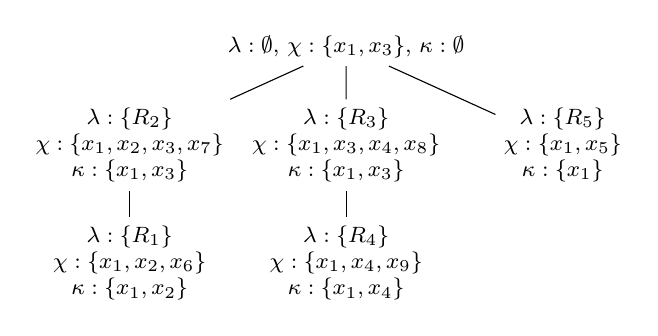
\begin{tikzpicture}[
			level 1/.style={level distance=1.25cm, sibling distance=2.75cm},
            level 2/.style={level distance=1.5cm, sibling distance=1.4cm},
            xscale=1,yscale=1
        ]
        \footnotesize
			\node { $\lambda: \emptyset$, $\chi: \{ x_1, x_3 \}$, $\kappa: \emptyset$ }
				child { node[align=center] {$\lambda: \{R_2\}$ \\ $\chi: \{ x_1, x_2, x_3, x_7 \}$ \\ $\kappa: \{ x_1, x_3 \}$} edge from parent[-]
                    child { node[align=center] {$\lambda: \{ R_1 \}$ \\ $\chi: \{ x_1, x_2, x_6 \}$ \\ $\kappa: \{ x_1, x_2 \}$} edge from parent[-] }
                }
                child { node[align=center] {$\lambda: \{ R_3 \}$ \\ $\chi: \{ x_1, x_3, x_4, x_8 \}$ \\ $\kappa : \{ x_1, x_3 \}$} edge from parent[-]
                        child { node[align=center] {$\lambda: \{ R_4 \}$ \\ $\chi: \{ x_1, x_4, x_9 \}$ \\ $\kappa: \{ x_1, x_4 \}$} edge from parent[-] }
                }
                    child { node[align=center] {$\lambda: \{ R_5 \}$ \\ $\chi: \{ x_1, x_5 \}$ \\ $\kappa : \{ x_1 \}$} edge from parent[-] }
                ;
		\end{tikzpicture}
        \vspace{-0.25\baselineskip}
        \caption{Meta-decomposition}
        \label{fig:complicated-meta}
    \end{subfigure}
    
    \vspace{0.5\baselineskip}
    
    \begin{subfigure}{.32\linewidth}
        \centering
        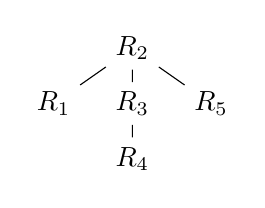
\begin{tikzpicture}[
			level distance=0.7cm,
			level 1/.style={sibling distance=1cm}
        ]
			\node { $R_2$ }
				child { node {$R_1$} edge from parent[-] }
                child { node {$R_3$} edge from parent[-]
                    child { node {$R_4$} edge from parent[-] }
                }
                child { node {$R_5$} edge from parent[-] } ;
		\end{tikzpicture}
        \vspace{-0.25\baselineskip}
        \caption{A join tree}
        \label{fig:complicated-jt1}
    \end{subfigure}
    \hfill
    \begin{subfigure}{.32\linewidth}
        \centering
        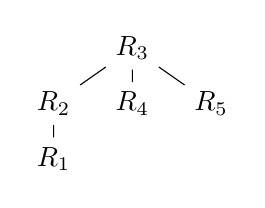
\begin{tikzpicture}[
			level distance=0.7cm,
			level 1/.style={sibling distance=1cm}
        ]
			\node { $R_3$ }
                child { node {$R_2$} edge from parent[-]
                    child { node {$R_1$} edge from parent[-] }
                }
				child { node {$R_4$} edge from parent[-] }
                child { node {$R_5$} edge from parent[-] } ;
		\end{tikzpicture}
        \vspace{-0.25\baselineskip}
        \caption{A second join tree}
        \label{fig:complicated-jt2}
    \end{subfigure}
    \hfill
    \begin{subfigure}{.32\linewidth}
        \centering
        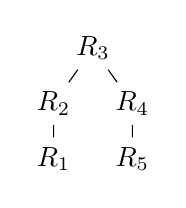
\begin{tikzpicture}[
			level distance=0.7cm,
			level 1/.style={sibling distance=1cm}
        ]
			\node { $R_3$ }
                child { node {$R_2$} edge from parent[-]
                    child { node {$R_1$} edge from parent[-]
                    }
                }
				child { node {$R_4$} edge from parent[-]
                    child { node {$R_5$} edge from parent[-] }
                };
		\end{tikzpicture}
        \vspace{-0.25\baselineskip}
        \caption{A third join tree}
        \label{fig:complicated-jt3}
    \end{subfigure}
    \end{minipage}
    \caption{Hypergraph, meta-decomposition, and three join trees of the query $Q_{\ref{ex:meta-complicated}}$ in \cref{ex:meta-complicated}}
    \label{fig:complicated}
\end{figure}


\end{example}


\subsection{Constructing Meta-Decompositions}

\begin{algorithm}
\caption{Constructing the meta-decomposition of an acyclic hypergraph} \label{alg:meta}
\SetKwInOut{Input}{input}
\SetKwInOut{Output}{output}
\SetKwInOut{Known}{known}
% \begin{multicols}{2}
\Input{An acyclic hypergraph $H$}
\Output{The meta-decomposition $M$ of $H$}
$H' \gets $ a copy of the input hypergraph $H$ with $V(H') = V(H)$ and $E(H') = E(H)$ \;
$V(M) \gets \emptyset$, $E(M) \gets \emptyset$ \;

\tcp*[l]{Reduction, creating the vertices in the meta-decomposition at the same time}
\While{$E(H')$ is not empty \label{alg:meta-while}} {
    \tcp*[l]{First check if it is possible to create minor nodes for mutually reducible hyperedges}
  \ForEach{maximal $S \subseteq E(H')$ such that $|S| > 1$, and, for all $e \in S$, $o(e, H')$ has the same value $o$ \label{alg-line:meta-minor-origins-sets}}{
    \ForEach{$e \in S$}{
        Add a node $p$ to $V(M)$ with $\lambda(p) = \set{e}$ if $e \in E(H)$, or $\lambda(p) = \emptyset$ if it is special, $\chi(p) = e$, and $\kappa(p) = o(e, H')$ \label{alg-line:meta-origin-node}, if such $p$ does not exist yet \;
        Remove $e$ from $E(H')$ \label{alg-line:meta-origin-remove} \;
    }
    Add a special hyperedge $e_m = o$ to $E(H')$ \label{alg-line:meta-add-special-edge} \;
  }
  $\mathcal{E} \gets$ the set of all ears in $E(H')$ \;

  \ForEach{$e \in \mathcal{E}$}{
    Add a new node $p$ to $V(M)$ with $\lambda(p) = \set{e}$ if $e \in E(H)$, or $\lambda(p) = \emptyset$ if it is special, $\chi(p) = e$, and $\kappa(p) = o(e, H')$, if such $p$ does not exist yet \label{alg-line:meta-ear-node} \;
    Remove $e$ from $E(H')$ \label{alg-line:meta-ear-remove} \;
    \If {there exists at least two vertices $p' \in V(M) \cup \mathcal{E}$ such that $\kappa(p') = \kappa(p)$ \label{alg-line:no-minor-check}} {
        Add a (minor) node $v$ to $V(M)$ with $\lambda(v) = \emptyset$, $\chi(v) = \kappa(p)$, and $\kappa(v) = \kappa(p)$, if such $v$ does not exist yet \label{alg-line:no-minor-create}\;
    }
  }

}
$r(M) \gets $ the node $p \in V(M)$ such that $\kappa(p) = \emptyset$ \;
\tcp*[l]{Generate the edges in the meta-decomposition}
\ForEach {non-root node $p \in V(M)$} {
    \If {there exists a (minor) node $q \in V(M)$ such that $\lambda(q) = \emptyset$ and $\chi(q) = \kappa(p)$ \label{alg-line:minor-origin-edge-cond}} {
        Add an edge $(q, p)$ in $E(M)$ \;
    } \Else( ) {
        Find the node $q \in V(M)$ such that $\kappa(p) \subseteq \chi(q)$ and $\kappa(p) \not\subseteq \kappa(q)$ \label{alg-line:phys-find-parent} \tcp*[r]{``highest'' possible parent}
        Add an edge $(q, p)$ in $E(M)$ \;
    }
}
\Return $M = (V(M), r(M), E(M), \lambda, \chi, \kappa)$ \;
\end{algorithm}

Similar to the original GYO algorithm~\cite{grahamGYO,DBLP:conf/compsac/YuO79}, a meta-decomposition can be constructed by a reduction-based algorithm, as shown in \cref{alg:meta}. In this algorithm, $o(e, H) = e \cap ( \cup (E(H) \setminus \set{e}) )$ denotes the set of overlapping vertices of hyperedge $e$ and the remaining hyperedges $E(H) \setminus \set{e}$.  As in the original GYO algorithm~\cite{grahamGYO,DBLP:conf/compsac/YuO79}, a hyperedge $e$ is \emph{reducible} (also called an \emph{ear}), if there exists another single hyperedge $e' \in E(H) \setminus \{ e \}$ such that $o(e, H) \subseteq e'$.  
The subsuming hyperedge $e'$ is called the \emph{witness}.
And, exceptionally, if there is only one hyperedge $e$ in the hypergraph, it is also considered an ear.
We note that the GYO algorithm removes exactly one ear (among possibly many) in each round, thereby establishing a total order of all hyperedge removal.
In contrast, Algorithm~\ref{alg:meta} \emph{simultaneously removes all ears in every round} until only a single hyperedge remains in the hypergraph. This process introduces only a partial order for all hyperedges, which \emph{maintains the flexibility to represent all possible ordering of ear removal, and hence all possible join trees}, through the resulting meta-decomposition.

\begin{example}
    For the star query $Q_{\ref{ex:star}}$ in \cref{ex:star}, the four hyperedges can be removed in any order in the standard GYO algorithm. For example:
    \begin{enumerate}[leftmargin=*]
        \item With the order $R_4$ (witness $R_3$) -- $R_3$ (witness $R_2$) -- $R_2$ (witness $R_1$) -- $R_1$, we obtain the first join tree in \cref{fig:star-jts}.
        \item With the order $R_4$ (witness $R_3$) -- $R_2$ (witness $R_1$) -- $R_3$ (witness $R_1$) -- $R_1$, we obtain the second join tree in \cref{fig:star-jts}.
    \end{enumerate}
    Furthermore, we note that we can also obtain the second join tree by keeping the order in (1) but only changing witnesses, namely $R_4$ (witness $R_3$) -- $R_3$ (witness $R_1$) -- $R_2$ (witness $R_1$) -- $R_1$.
\end{example}


To address this source of variation, in every round, our algorithm first handles such cases where some edges $ e_1, \dots, e_n$ are \emph{mutually reducible}, i.e., $o(e_1, H) = \dots = o(e_n, H) = o$ (Lines \ref{alg-line:meta-minor-origins-sets}--\ref{alg-line:meta-add-special-edge}).  
(For example, in the case of $Q_{\ref{ex:star}}$, all pairs among $R_1$, $R_2$, $R_3$, and $R_4$ are mutually reducible.)
The algorithm creates a minor node $p$ with $\chi(p) = o$ if such a node does not yet exist, and then removes $e_1, \dots, e_n$ from the hypergraph.  We then add a special hyperedge $e_m = o$, which conceptually corresponds to the minor node, back to the hypergraph, so that the acyclicity of $H$ is preserved. The rationale for adding such an $e_m$ can be illustrated by the following example:

\begin{example}
    \label{ex:special-hyperedge}
    Consider the query
    \begin{align*}
        Q_{\ref{ex:special-hyperedge}} \gets \pi_{\emptyset} (& R_1[x_1, x_2, x_3, x_4] \bowtie R_2[x_1, x_2, x_5] \bowtie R_3[x_1, x_3, x_6] \bowtie R_4[x_2, x_3, x_7] \bowtie R_5[x_1, x_2, x_3, x_8]),
    \end{align*}
    which is similar to \cref{ex:123-12-13-23-intro} but contains an additional relation $R_5$. In this case, at the beginning, $R_1$ and $R_5$ are both ears and mutually reducible, as $o(R_1, H) = o(R_5, H) = \{ x_1, x_2, x_3 \}$. However, if we simply remove both $R_1$ and $R_5$ at the same time, \emph{the remaining hyperedges, $R_2$, $R_3$, and $R_4$, form a cyclic hypergraph}. But, if we add $e_m = o(R_1, H) = o(R_5, H) = \{ x_1, x_2, x_3 \}$, then $e_m$, $R_2$, $R_3$, and $R_4$ still form an acyclic query, and the algorithm can proceed to pick $R_2$, $R_3$, and $R_4$ as ears, before $e_m$ is picked and removed at the very end.
\end{example}

We formalize this idea as follows:

\begin{proposition} \label{lem:add-back-minor}
    Given an acyclic hypergraph $H$, if there exists a set of distinct ears $S = \{ e_1, \dots, e_n \} \subseteq E(H)$ $(n \geq 2)$ such that $o(e_1, H) = \dots = o(e_n, H) = o$, then, the hypergraph $H'$, with $E(H') = (E(H) \setminus S) \cup \{ o \}$ and $V(H') = \cup E(H')$, is acyclic.
\end{proposition}

% \begin{sketch}
%     In the GYO algorithm for $H$, since $o(e_1, H) = o(e_2, H) \subseteq e_2$, $e_1$ is an ear and can already be removed, with $e_2$ being its witness. So, there exists a join tree $T$ of $H$ where there is a leaf node $p_1$ with $\lambda(p_1) = \{ e_1 \}$, and its parent $p_2$ has $\lambda(p_2) = \{ e_2 \}$. If we merge $p_1$ and $p_2$ into a single node $p_m$ with $\lambda(p_m) = \{ o(e_1, H) \}$ to obtain a new tree $T'$, $T'$ is a join tree of $H'$.
% \end{sketch}

In each round, the algorithm then finds and removes the set $\mathcal{E}$ of all ears of $H'$.
For each $e \in \mathcal{E}$, we create a node $p$ with set $\kappa(p) = o(e, H')$.  
$p$ may be either physical or minor, depending on whether $e$ is a hyperedge in $H$ or a special hyperedge created while removing mutually reducible hyperedges.
% Then, these ears are all removed from the hypergraph, and the next round of reduction can be performed.  
During the procedure, the algorithm creates minor nodes whenever necessary (Lines~\ref{alg-line:meta-origin-node}, \ref{alg-line:meta-ear-node}, and \ref{alg-line:no-minor-check}--\ref{alg-line:no-minor-create}).

This algorithm has the following guarantee of asymptotic complexity:

\begin{theorem} \label{thm:meta-complexity}
    \cref{alg:meta} terminates in time $O(|E(H)|^3)$.
\end{theorem}

\begin{sketch}
    The key observations are (1) that the size $|E(H')|$ decreases by at least one in each iteration of the while-loop (\cref{alg:meta-while}), and (2) that, in each iteration of the while loop, all sets $S$ (\cref{alg-line:meta-minor-origins-sets}) can be enumerated in $O(|E(H')|) = O(|E(H)|)$ time, if we maintain a hash map that maps each $o \subseteq V(H')$ to all hyperedges $e \in E(H')$ such that $o(e, H') = o$, which is updated whenever a hyperedge $e$ is added or removed from $E(H')$.
\end{sketch}

We show the correctness of the algorithm:

\begin{theorem} \label{thm:meta-correct}
    Given an acyclic query with an acyclic hypergraph $H$, \cref{alg:meta} returns a valid meta-decomposition of $H$.  
\end{theorem}

Finally, we note that meta-decompositions are highly space-efficient. They only require space linear to the size of the hypergraph.

\begin{theorem} \label{thm:meta-size}
    In the meta-decomposition $M$ of an acyclic hypergraph $H$ as constructed by \cref{alg:meta}, the number of vertices $|V(M)|$ and the number of edges $|E(M)|$ are $O(|E(H)|)$.
\end{theorem}

\begin{sketch}
    Vertices in $M$ are either physical or minor. We create one physical node per hyperedge in $E(H)$. For minor nodes, we note that each minor node has fan-out at least 2, meaning there must be at least two edges incident to each minor node.
\end{sketch}

\subsection{Join Tree Enumeration}
\label{sec:enum}

The meta-decomposition allows one to efficiently enumerate all possible join trees of an acyclic query, as we show with an algorithm in this section. This not only serves as proof of the universality of this representation but also provides a powerful approach to enumerating join trees, which could be of great help to other structure-based methods that require doing so.

As an intuition, we can observe that the distinct join trees of the same hypergraph may differ in the following ways:
\begin{enumerate}[leftmargin=*]
    \item \textbf{``Re-branching''.} If a vertex $p$ in a join tree has children $c_1$ and $c_2$ such that
    $\chi(c_1) \cap \chi(p) \subseteq \chi(c_2)$,
    then $c_1$ could have been a child of $c_2$ without violating any condition. In the meta-decomposition, condition \ref{H4} ensures that $c_1$ is positioned at the highest possible node. When enumerating join trees, we can make $c_1$ a child of $c_2$ if $\kappa(c_1) \subseteq \chi(c_2)$, without violating any condition. The join tree in \cref{fig:complicated-jt3} based on the meta-decomposition in \cref{fig:complicated-meta} from \cref{ex:meta-complicated} demonstrates such a case, where $R_5$ could be a child of any one of $R_1$, $R_2$, $R_3$, and $R_4$.
    \item \textbf{Rerooting.} A rerooting of a join tree is still a valid join tree.
    \item \textbf{Mutually reducible relations.} If multiple relations share some exact same set of attributes, they can be connected in arbitrary tree structures. This situation is represented by minor nodes in meta-decompositions. An example is the root node with $\chi$-label $\{ x_1 \}$ in \cref{fig:star-meta} for \cref{ex:star}, based upon which we should be able to enumerate, among others, the join trees in \cref{fig:star-jts}.
\end{enumerate}

These alternatives should be considered to enumerate all join trees, and the meta-decomposition retains all the necessary information to facilitate this. \cref{alg:enum} is an algorithm to enumerate all join trees. For each node in the meta-decomposition starting from the root, it recursively enumerates all possible join trees given by the subtree rooted at each of its children (Lines \ref{alg-line:enum-for-each-child}--\ref{alg-line:enum-subtrees}), and then enumerates all possible ways to combine these join trees into one. For minor nodes $r$, we find its neighbors that share the common set of attributes given by $\chi(r)$ (\cref{alg-line:enum-origin-set}) and generate all possible distinct structures of join trees, where each vertex will be replaced by the join tree for a subtree given by a neighbor. (At this point, we consider all rerootings of the same tree as identical.) At the very end of this algorithm, we return all combined join trees we obtain, and it remains only to collect all rerootings.  Due to space constraints, we omit some lower-level details, e.g., the exact steps for combining sub-join trees and algorithms to enumerate all trees and rerootings without repetition. The full details are given in the \arxivorappendix.

\begin{algorithm}
\small
\caption{Enumerating all join trees based on a meta-decomposition} \label{alg:enum}
\SetInd{0.5em}{0.6em}
\SetKwInOut{Input}{input}
\SetKwInOut{Output}{output}
\SetKwInOut{Known}{known}
\SetKwProg{Fn}{Function}{:}{}
\SetKwFunction{enumRec}{$\mathsf{enumRec}$}
\Input{A meta-decomposition $M = (V(M), r(M), E(M), \lambda, \chi, \kappa)$}
\Output{All join trees of the hypergraph induced by $M$}

\Fn{\enumRec{$v$: a node on $M$}}{

$\mathcal{C} \gets $ set of children $c$ of $v$ on $M$, sorted by partial order $\supseteq$ on $\kappa(c)$ \;
\ForEach{$c \in \mathcal{C}$ \label{alg-line:enum-for-each-child}} {
    $\mathcal{T}_c \gets$ all rerootings $T_c'$ of all trees $T_c$ returned by $\mathsf{enumRec}(c)$ such that $\kappa(c) \subseteq \chi(r(T_c'))$ \label{alg-line:enum-subtrees} \;
}

\If(\tcp*[f]{minor node}){$\lambda(v) = \emptyset$ \label{alg-line:enum-minor-cond}} {
    $\mathcal{C}_{\sf origin} \gets \{ c \in \mathcal{C} : \kappa(c) = \chi(v) \}$ \label{alg-line:enum-origin-set} \tcp*[r]{They can be found at the head of the sorted $\mathcal{C}$}
    \If{$\kappa(v) = \chi(v)$}{
        $\mathcal{T} \gets $ all non-isomorphic trees with vertices $\mathcal{C}_{\sf origin} \cup \{ v \}$, all rerooted to $v$
        \label{alg-line:enum-minor-dummy} \;
        \tcp*[r]{The minor node $v$ will eventually be replaced on \cref{alg-line:enum-simplified-dummy-replace} by the parent of $r$}
    } \Else(\tcp*[f]{$\kappa(v) \neq \chi(v)$, the parent should not participate}) {
        $\mathcal{T} \gets $ all non-isomorphic trees with vertices $\mathcal{C}_{\sf origin}$ \label{alg-line:enum-minor-no-dummy} \;
    }
            $\mathcal{T} \gets $ set of trees $T'$ that can be obtained from some $T \in \mathcal{T}$, where each $c \in V(T)$, in bottom-up order, is replaced by some $T_c \in \mathcal{T}_c$, and, for each non-root $c \in V(T)$ with parent $p$, $T_c$ could be attached as a child of any $u \in V(T_p)$ such that $\kappa(c) \subseteq \chi(u)$ \;
    $\mathcal{C}_{\sf proper} \gets \mathcal{C} \setminus \mathcal{C}_{\sf origin}$, preserving the order \tcp*[r]{The set of children $c$ such that $\kappa(c) \subsetneq \chi(v)$}
} \Else {
    $\mathcal{T} \gets $ a set of one tree with one vertex $v$ only \label{alg-line:enum-physical-root} \;
    $\mathcal{C}_{\sf proper} \gets \mathcal{C}$, preserving the order \;
}
\ForEach {child $c \in \mathcal{C}_{\sf proper}$ in order,
    $T_c \in \mathcal{T}_c$} {
        \If{$\lambda(c) = \emptyset$ and $\kappa(c) = \chi(c)$}{
            \tcp*[r]{The root of $T_c$ would be a minor node from \cref{alg-line:enum-minor-dummy}. We find a parent of each of its children.}
            $\mathcal{T} \gets $ set of trees $T'$ that can be obtained from some $T \in \mathcal{T}$, where for each child $d$ of $r(T_c)$, we attach the subtree rooted at $d$ as a child of some $u \in V(T)$ such that $\kappa(d) \subseteq \chi(u)$ \label{alg-line:enum-simplified-dummy-replace} \;
            
        } \Else {
            $\mathcal{T} \gets $ set of trees $T'$ that can be obtained from some $T \in \mathcal{T}$, where $T_c$ is attached as a child of some $u \in V(T)$ such that $\kappa(c) \subseteq \chi(u)$ \;
        }
}

\Return{$\mathcal{T}$} \;
    
}

\Return{all rerootings of all trees returned by $\mathsf{enumRec}(r(M))$ } \;
\end{algorithm}

\begin{example}
    Consider again the query $Q_{\ref{ex:meta-complicated}}$ in \cref{ex:meta-complicated}. Its meta-decomposition is shown in \cref{fig:complicated-meta}. Let the root node be $r$, and we use $v_1, \dots v_5$ to denote the nodes such that $\lambda(v_i) = \{ R_i \}$.
    The root node $r$ is a minor node, with $\chi (r) = \{ x_1, x_3 \}$.
    We start by enumerating all possible join trees induced by the subtrees of the meta-decomposition, rooted at each child of $r$.
    For the subtree with $v_2$ and $v_1$, there is only one valid join tree, rooted at $v_2$, which has one child $v_1$. It is not possible to reroot to $v_1$ because $\kappa(v_2) = \{ x_1, x_3 \} \not\subseteq \chi(v_1)$. The case is similar for the subtree with $v_3$ and $v_4$. And the subtree with $v_5$ induces only one join tree with one node $v_5$.
    Since $v_2$ and $v_3$ (and not $v_5$) have $\kappa(v_2) = \kappa(v_3) = \chi(r) = \{ x_1, x_3 \}$, we enumerate all possible skeleton tree structures with vertices $v_2$ and $v_3$.
    There are only two such trees, each of which contains one edge connecting $v_2$ and $v_3$, and they are rerootings of each other.
    For each tree, we replace $v_2$ and $v_3$ by their induced join tree.
    In the end, we have one child $v_5$ with $\kappa(v_5) \subsetneq \chi(r)$.
    It can be a child of any node $v$ such that $\kappa(v_5) \subseteq \chi(v)$. In this example, it can, in fact, be a child of any other node.
    \cref{fig:complicated-jt1} is a join tree where the skeleton tree structure is rooted at $R_2$, and $R_5$ is attached as a child of $R_2$. \cref{fig:complicated-jt2} is a similar example where the skeleton is rooted at $R_3$, and $R_5$ is attached as a child of $R_3$. And \cref{fig:complicated-jt3} is based on the same skeleton as for \cref{fig:complicated-jt2}, but $R_5$ is attached as a child of $R_4$ instead of $R_3$.
\end{example}

We claim that this algorithm is both correct (producing valid join trees) and complete (enumerating all possible join trees).

\begin{theorem}[Correctness]
\label{the:correctness}
    Given a meta-decomposition $M$ of an acyclic hypergraph $H$, all trees $T$ output by \cref{alg:enum} are valid join trees of $H$.
\end{theorem}

\begin{theorem}[Completeness] \label{thm:enum-complete}
    Given a meta-decomposition $M$ of an acyclic hypergraph $H$, \cref{alg:enum} enumerates all possible join trees of $H$.
\end{theorem}

As is detailed in the proof of \cref{thm:enum-complete}, for each join tree, we can pinpoint exactly one way in which it is enumerated by the algorithm based on the meta-decomposition. Noting that the number of children of each node on a meta-decomposition is bounded by the fan-out, we get the following guarantee of enumeration delay.

\begin{theorem}[Time complexity]
    Given a meta-decomposition $M$ of an acyclic hypergraph $H$, \cref{alg:enum} enumerates all possible join trees of $H$ in an amortized delay of $O(f(M) \cdot|V(H)|)$.
\end{theorem}
